\subsection{Analiza udostępnianych domen }
W kolejnym badaniu chciano sprawdzić jakie zewnętrzne serwisy są udostępniane przez analizowane konta. Celem, podobnie jak w\,badaniu powyżej, było sprawdzenie czy istnieją relacje między badanymi kontami. W\,tym przypadku chciano zbadać, czy istnieją takie wspólne domeny, które są udostępniane przez analizowane konta, i\,jeśli tak to czy te konta należą do jednej klasy czy różnych.
W celu analizy takich zależności pobrano wszystkie linki url które znajdowały się w\,publikowanych przez badane konta postach. Aby ujednolicić 39 tysięcy pobranych url, skupiono się jedynie na domenach do których te linki prowadzą. Dodatkowo najpierw należało rozszerzyć niektóre z\,linków, ponieważ duża część z\,nich była poddana działaniu serwisów skrócających url. 
\par
Z pobranych danych stworzono graf dwudzielny, gdzie pierwszym zbiorem są analizowane konta a\,drugim domeny przez nie udostępniane w\,postach. Aby domena znalazła się w\,tym zbiorze musiała być udostępniona przez jakieś konto przynajmniej 30 razy w\,analizowanym zbiorze. Łuk istnieje między nimi, gdy konto udostępniało w\,swoich postach daną domenę. 
\begin{figure}[!h]
	\centering 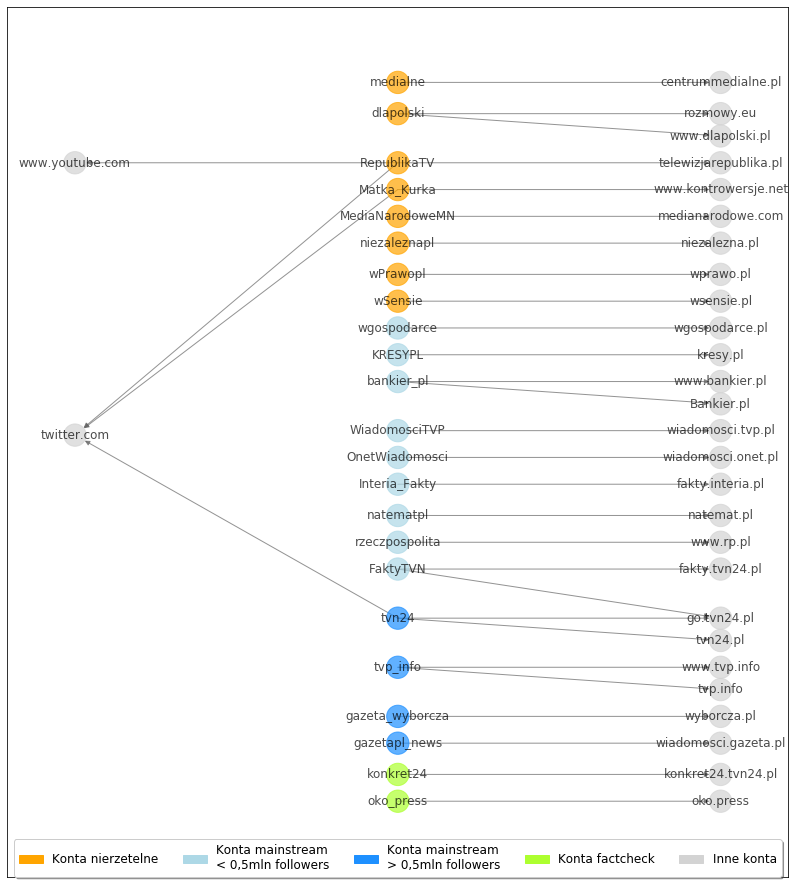
\includegraphics[width=1.0\linewidth]{img/results/connectionwithlikns.png}
	\caption{Sieć udostępnień domen przez konta z\,podziałem na klasy} \label{fig:connectedlinks}
\end{figure}
Dzięki wizualizacji grafu ukazującego udostępnienia domen przez analizowane konta \ref{fig:connectedlinks} można łatwo zobaczyć, że udostępnianie zewnętrznych domen w\,postach na tweeterze w\,omawianym przypadku sprowadza się prawie wyłącznie do udostępniania serwisu, do którego to konto należy. Jedyną domeną która jest udostępniana przez kilka kont jest twitter.com, znajdują się tam linki do innych tweetów, których zapewne nie chciano bezpośrednio udostępnić. 